\section{Lecture 10, Neural Coding}
Problem of neural coding: A single neuron spikes in a probabilistic way. Neglecting the duration of an action potential (~1ms) and differences in maximal amplitude and shape, action potentials can be stereotyped and therefore be thought of as a random variable. Therefore, statistical methods are needed to get meaningful statements. In the following, a ``run'' refers to a random experiment, in which a neuron can respond (several times) to a stimulus.
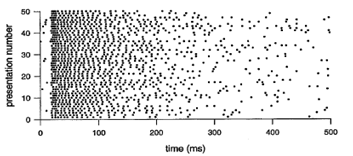
\includegraphics[width=10cm]{neuroinf_spikeruns.png}\\
Abbreviation: (S$|$M)N(S$|$M)R = (Single$|$Multiple) Neuron, (Single$|$Multiple) Run\\
\subsection{Neuronal Rate Codes}
Neuronal rate codes rely on the spike rate as information carrier. The different methods show how such a rate can be computed.\\
\begin{longtable}{p{4cm}p{15cm}}
Neuronal gain function (SNSR)	& Output spike rate = f(input current). The mean spike rate is determined by a temporal average over the spikes of a neuron in a run.\\
Peri-Stimulus Time Histogram (SNMR)	& Average over several runs. No temporal average is taken. The probability of a spike ($\Leftrightarrow$ firing rate) depends on the time.\\
Rate as a function of stimulus	& 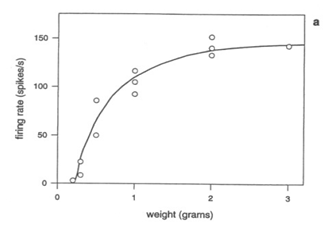
\includegraphics[width=10cm]{neuroinf_ratestimulus1.png}\\
Adaption to stimulus		& 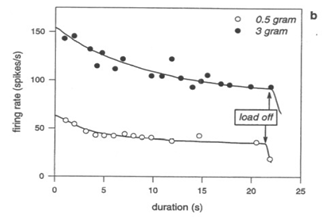
\includegraphics[width=10cm]{neuroinf_ratestimulus2.png}\\
\textbf{Tuning curves}		& Neurons of any kind often have a preferred stimulus, i.e. the spike rate is extraordinarily high for a certain stimulus. E.g. the peak firing rate of the ``blue'' photoreceptor in the retina is for wavelengths around 450 nm (blue color) or head direction cells in rats or ``Jennifer Aniston cells'' That means, a neuron can encode a certain (very exact) information.\\
What can a single neuron encode (examples)	& \begin{itemize}
                               	  	\item Placement (Rat hippocampus): Fires whenever rat enters a particular region in its environment
					\item Head-direction: Fires whenever rat's head points to a specific direction (compass)
					\item Anything about Jennifer Aniston
                               	  \end{itemize}\\
Topographic maps		& In the CNS, many neurons which have similar preferred stimuli, are grouped together, i.e. the distances between them are small. For example, there are topographic maps for the visual system, the auditotory system and so on. It makes sense that the neurons build clusters between neurons which will be highly interconnected.\\
Pros and Cons			& \begin{tabular}[t]{p{7cm}p{7cm}}
				    +: Easy to understand and measure	& -: No timing effects\\
									& -: The behavioural response time is shorter than the integration time\\
									& -: Tuning curves might be misleading, because more than one stimulus could be encoded.
				  \end{tabular}\\
\end{longtable}
\subsection{Population Rates (MNSR)}
\begin{tabular}{p{4cm}p{15cm}}
Population	& A population is a family of neurons which react to the same type of stimulus but have different peak reactions. (e.g. Photoreceptor cells) As an individual neuron is too noisy and therefore unreliable, a population of neurons levels out these noises statistically.\\
Rate		& The rate is determined by an average over equivalent neurons in a single run.\\
Statistics	& For the photoreceptor cells for example, it makes no sense to average over the firing rates. Rather an average over the encoded information (the color wavelength), weighted with the photoreceptor's spike rate is meaningful. (E.g. Activation of S and L photoreceptor results in a color somewhere on the purple line)\\
Examples	& Neuron for sensing movement directions, neuron for sensing wind directions
\end{tabular}
\subsection{Neuronal Event Codes}
Sometimes, the precise timing of a spike encodes information (for example spike-time-dependent plasticity). Then, coding relying solely on firing rates is insufficient. Therefore, neuronal event codes depend on the timing of spikes.\\
\begin{tabular}{p{4cm}p{15cm}}
Time-to-first-spike codes	& Instead of a firing rate, the time to the first spike is the information carrier. Relationship to rate codes: High rate implies fast firing\\
Pros and Cons			& \begin{tabular}[t]{p{7cm}p{7cm}}
				    +: Very fast and efficiently measured	& -: Requires reference signal\\
										& -: Susceptible to noise\\
				  \end{tabular}\\
Local field potential		& Dominated by dendritic synaptic activity, reflects the integration of membrane currents in a local region. Interesting if LFP high, but no firing takes place.\\
\end{tabular}
\subsection{Stimulus reconstruction}
\begin{itemize}
	\item Whole stimulus reconstruction may not be relevant.
	\item Particular features may be encoded better (more precisely by a neuron, e.g. ``Jennifer Aniston Neuron'') than others.
	\item Cells may respond to only particular aspects of stimulus.
	\item Or respond to multiple aspects of stimulus.
	\item Artificial stimuli used for studies may be predictable.
\end{itemize}